\documentclass[a4paper,11pt,twoside]{report}
\usepackage[nodisplayskipstretch]{setspace}
\usepackage{mathtools}
\usepackage{etoolbox}
\usepackage{layout}
\usepackage[round]{natbib}
\usepackage{listings}
\usepackage{Packages}
\usepackage{wrapfig}
\usepackage{graphicx}
\usepackage[framed,numbered,autolinebreaks,useliterate]{Listings}
%\usepackage{SIunits}
%\addunit\decibelm{dBm}
\usepackage[belowskip=-22pt,aboveskip=0pt]{caption}
 
\setlength{\intextsep}{11pt}


\addto\captionsbritish{\renewcommand{\contentsname}{Table of Contents}}

%\linenumbers
\usepackage{enumitem}
\newcommand{\shortdoctitle}{Fall Detection}
\newcommand{\doctitle}{Fall Detection Using Wi-Fi Signals}
\newcommand{\docsubtitle}{}


\newcommand{\authorone}{Robert Keenan}
\newcommand{\sauthorone}{15333066}
\newcommand{\keywords}{keyword1, keyword2, keyword3}
\newcommand{\version}{First version}
\newcommand{\monthYear}{January 2020}

\newcommand{\firstCommitteeMember}{Dr. Nam Tran}

\author{\me}
\setlength{\parindent}{17pt}
\hypersetup
{
    pdfauthor   = {Robert Keenan},
    pdftitle    = {\shortdoctitle},
    pdfsubject  = {\doctitle}
}
\linespread{2}
%\doublespacing
\begin{document}

\begin{titlepage}
\begin{center}

\includegraphics[height=4cm]{Figures/ucd_logo.png} \\
\LARGE
University College Dublin \\
\Large
School of Electrical \& Electronic Engineering \\
\large
\underline{ME Interim Report}
%\vspace*{10cm}


%\setlength{\TPHorizModule}{1mm}
%\setlength{\TPVertModule}{\TPHorizModule}

%\newlength{\backupparindent}
%\setlength{\backupparindent}{\parindent}
%\setlength{\parindent}{0mm}
\huge
\textbf{\doctitle \\}
\begin{singlespacing}
    \Large
    \authorone \\
    \sauthorone \\
\end{singlespacing}
\vfill
\large
\underline{Supervisor:} \\
\firstCommitteeMember \\



\large
Dublin, \monthYear \\

%\setlength{\parindent}{\backupparindent}
\end{center}
\end{titlepage} 
\clearpage


\normalsize

%\chapter*{Abstract}\label{chapter:Abstract}
%\setcounter{page}{0}
%\pagenumbering{roman}
%\addcontentsline{toc}{chapter}{Abstract}
%Text

\begin{singlespacing}
    \tableofcontents
\end{singlespacing}

%\linespread{2}
\doublespacing
\chapter{Introduction}\label{chapter:Introduction}
\setcounter{page}{0}
\pagenumbering{arabic}
Falls are one of the leading causes of fatal and non-fatal injuries especially for elderly people in today's society. Quick response is vital to reducing the long-term effects on the victim physically, emotionally and mentally \citep{dangerousFalls,stokesFall}. Falls have been one of leading cause of injuries across all age groups placing a strain on health and financial systems around the world. \par
As a result, an efficient, accurate and cost effective detection system needs to be implemented for a variety of environments. Over 50\% of falls for the 65+ age group (1/3 experience a fall at least once a year) occur in their home so a solution that is \textbf{cheap, accurate, privacy-focused} and \textbf{easily installed} is needed \citep{medicalFall, stokesFall}. 
Personally, I have seen the effects falls can have on an elderly person and the fear induced in a fall victim post-treatment can deem them unable to live alone again. \citep{fearFall} \par
There are a number of solutions on the commercial market today which can be divided into a broad number of categories: Wearables, Visual, Ambient Environment. Products on the market in these categories include the Apple Watch, cameras, accelerometer belts, floor vibration sensors and infrared devices. \textbf{Privacy} is a key issue that needs to be addressed across the world in the next decade. Therefore, it was a key aim of my project to keep it as privacy oriented as possible. Many of the current solutions on the market suffer from privacy issues especially in such a sensitive environment as somebody's home. Many of these off-the-shelf solutions require \textbf{Direct Line of Sight (LOS)} to the person in the room to detect a fall. No obstacles can be in the way of the detection apparatus or a fall may not be detected by the system. This is especially useless in a busy household environment with many obstacles. All of these existing solutions are \textbf{very expensive} to buy and implement such as the Apple Watch, specialist cameras and Man-Down alarms. Another issue arises as elderly people are not inclined to wear them as they hinder them from daily activities and can feel like a chore to keep them charged/around their neck or waist. This results in a lot of people refusing to wear them which is clearly unsatisfactory as a solution. More complex solutions such as Computer Vision cameras require \textbf{high processing power} as the calculations and classification operations needed for the sheer amount of data recovered in any of these fall detection experiments. \par
Therefore, I propose a Wi-Fi based solution utilising commercial off the shelf (COTS) Wi-Fi network cards providing a cheap, highly accurate and non-intrusive fall detection system for the home and other environments. A fall is detected accurately and privately due to the rich multi-path environment that exists between a number of transmitting and receiving antennas. \par
\begin{comment}Previous research papers have explored the use of the Channel State Information (CSI) of a WLAN Channel for fall detection.\end{comment} 
The aims of the project/project plan are as follows: 
\vspace{-11pt}
\begin{itemize}[noitemsep, topsep=0pt]
\item Gain a strong understanding and background of CSI in the \textit{IEEE802.11n} Wi-Fi standard 
\item Build an initial system which can collect CSI using the Intel Wi-Fi Link 5300 NIC for a range of Transmitter-Receiver setups
\item Obtain CSI data for a range of human activities which would be typical in home/workplace environments
\item Design, build and test signal processing algorithms to clean the CSI data obtained for fall detection under various conditions
\item Design, implement and test various Machine Learning/Classification algorithms for fall detection for a target fall detection rate of $>$90\%
\end{itemize}
\begin{comment}
\begin{center}
\begin{tabular}{|c||p{10cm}|}
 \hline
 \multicolumn{2}{|c|}{\textbf{Project Timeline}} \\
 \hline
 \bfseries Date & \bfseries Task to be completed \\
 \hline
 19/09/19 & Allocation of Projects \\
 23/09 - 14/10 & Research OFDM, 802.11n, CSI \& Current State of the Art \\
 14/10 - 28/10 & Gather CSI data using Intel NIC under various activities, conditions \& environments \\ 
 28/10 - 18/11 & Researching, developing \& implementing signal processing algorithms to clean the CSI data for feature extraction \\
 26/11 & Interim Presentation \\
 27/11 - 6/12 & Gather data under more use cases \\
 03/01/20 - 15/01/20 & Identify features for activity segmentation of CSI data \\
 15/01 - 19/01 & Obtain much larger CSI datasets ($>$15mins of data) \\
 20/01 & Interim Report submission \\
 22/01 - 29/01 & Implement Activity Segmentation methods \\
 01/02 - 28/02 & Research, design \& implement different classification methods for fall detection \\
 29/02 - 22/03 & Test and tune classification methods for optimal fall detection accuracy \\
 27/03 & Conference Paper and Critique submission \\
 24/04 & Final Project Report Submission \\
 \hline
\end{tabular}
\end{center}
\end{comment}

\chapter{Literature Review}\label{chapter:Literature Review}
\section{Initial Theory \& Background}
\subsection{WLAN Channel Model}
\textbf{Give info on the wireless channel model in terms of the h matrix and more. what happens if i scale it to a mimo system and what the h matrix looks like then} \\\\
%%%%%%%%%%%%%%%%%%%%%%%%%%%%%%%%%%%%%%%%%%%%%%%%%%%%%%%%%%%%%%%%%%%%%





%%%%%%%%%%%%%%%%%%%%%%%%%%%%%%%%%%%%%%%%%%%%%%%%%%%%%%%%%%%%%%%%%%%%%
%%%%%%%%%%%%%%%%%%%%%%%%%%%%%%%%%%%%%%%%%%%%%%%%%%%%%%%%%%%%%%%%%%%%%
\subsection{Channel State Information (CSI)}
\textbf{This is an estimation of the channel matrix H and is split into a different number of subcarriers depending on the bandwidth of the channel.From this we can obtain a characteristic of how the channel is behaving at a certain time. Speak about RSSI in the context of other papers and papers on indoor localisation and why it isnt correct to use it. Give the diagram from my presentation of the scattering signal} \\\\
%%%%%%%%%%%%%%%%%%%%%%%%%%%%%%%%%%%%%%%%%%%%%%%%%%%%%%%%%%%%%%%%%%%%%






%%%%%%%%%%%%%%%%%%%%%%%%%%%%%%%%%%%%%%%%%%%%%%%%%%%%%%%%%%%%%%%%%%%%%
%%%%%%%%%%%%%%%%%%%%%%%%%%%%%%%%%%%%%%%%%%%%%%%%%%%%%%%%%%%%%%%%%%%%%
\subsection{Obtaining CSI information}
\textbf{How do we obtain CSI information, csi information requires beamforming to be activated. we can use the Linux CSI tool developed with Intel and Microsoft and talk about how it returns data and link to the document that released it} \\\\
%%%%%%%%%%%%%%%%%%%%%%%%%%%%%%%%%%%%%%%%%%%%%%%%%%%%%%%%%%%%%%%%%%%%%




%%%%%%%%%%%%%%%%%%%%%%%%%%%%%%%%%%%%%%%%%%%%%%%%%%%%%%%%%%%%%%%%%%%%%
%%%%%%%%%%%%%%%%%%%%%%%%%%%%%%%%%%%%%%%%%%%%%%%%%%%%%%%%%%%%%%%%%%%%%
\section{Related Work \& Existing Fall Detection Systems}
\textbf{In this section, talk about the current work in the area and what they did to get any of it to work. However, then look at how each of them gathered the data classified after activity segmentation} \\\\
%%%%%%%%%%%%%%%%%%%%%%%%%%%%%%%%%%%%%%%%%%%%%%%%%%%%%%%%%%%%%%%%%%%%%






%%%%%%%%%%%%%%%%%%%%%%%%%%%%%%%%%%%%%%%%%%%%%%%%%%%%%%%%%%%%%%%%%%%%%
%%%%%%%%%%%%%%%%%%%%%%%%%%%%%%%%%%%%%%%%%%%%%%%%%%%%%%%%%%%%%%%%%%%%%
\subsection{Justification for Fall Detection Systems}
\textbf{talk here about the need for fall detection systems due to the amount of people falling each year/the amount of people who are causing the financial and health systems to be overloaded with falls} \\\\
%%%%%%%%%%%%%%%%%%%%%%%%%%%%%%%%%%%%%%%%%%%%%%%%%%%%%%%%%%%%%%%%%%%%%




%%%%%%%%%%%%%%%%%%%%%%%%%%%%%%%%%%%%%%%%%%%%%%%%%%%%%%%%%%%%%%%%%%%%%
%%%%%%%%%%%%%%%%%%%%%%%%%%%%%%%%%%%%%%%%%%%%%%%%%%%%%%%%%%%%%%%%%%%%%
\subsection{Wearable Approaches}
\textbf{Wearable approaches such as Accelerometers, phones, man down and what they have advantages and disadvantages. why they arent used. the privacy issues, the issue with people not wearing them} \\\\
%%%%%%%%%%%%%%%%%%%%%%%%%%%%%%%%%%%%%%%%%%%%%%%%%%%%%%%%%%%%%%%%%%%%%





%%%%%%%%%%%%%%%%%%%%%%%%%%%%%%%%%%%%%%%%%%%%%%%%%%%%%%%%%%%%%%%%%%%%%
%%%%%%%%%%%%%%%%%%%%%%%%%%%%%%%%%%%%%%%%%%%%%%%%%%%%%%%%%%%%%%%%%%%%%
\subsection{Ambient Environment Approaches} 
\textbf{The ambient environment issues in terms of infrared, floor vibration and sound sensors. sound is an iffy one because of how busy some of these environments are such as in a home. the TV could be on and there could be a false detection......floor vibration is expensive and useless tbh} \\\\
%%%%%%%%%%%%%%%%%%%%%%%%%%%%%%%%%%%%%%%%%%%%%%%%%%%%%%%%%%%%%%%%%%%%%




%%%%%%%%%%%%%%%%%%%%%%%%%%%%%%%%%%%%%%%%%%%%%%%%%%%%%%%%%%%%%%%%%%%%%
%%%%%%%%%%%%%%%%%%%%%%%%%%%%%%%%%%%%%%%%%%%%%%%%%%%%%%%%%%%%%%%%%%%%%
\subsection{Fall Detection using CSI}
\textbf{talk about any of the papers that have used it. first one will be WiFall, go through they use amplitude, how they get the data and how they organise it into different column arrays....talk about the frequency diversity and how it is actually impossible to limit it down, talk about the typical activity segmentation (what they use for activity detection), what they use for the classification and talk about how it is simply a binary decision \\ With Rt fall the decision is used to use the phase difference as it is a much more fine grainer use and this can be seen from Fila, E-eyes, perceiving accurate phase, what they used for each of it to get data or a model to train } \\\\
%%%%%%%%%%%%%%%%%%%%%%%%%%%%%%%%%%%%%%%%%%%%%%%%%%%%%%%%%%%%%%%%%%%%%





%%%%%%%%%%%%%%%%%%%%%%%%%%%%%%%%%%%%%%%%%%%%%%%%%%%%%%%%%%%%%%%%%%%%%
%%%%%%%%%%%%%%%%%%%%%%%%%%%%%%%%%%%%%%%%%%%%%%%%%%%%%%%%%%%%%%%%%%%%%
\subsection{Activity Segmentation}
\textbf{Now that I have considered each of the ways of doing it, how can i spot an activity of falling vs any of the others. Use RT Fall for this and WiFall....talka about the function that RTFall used and also how they can determine a fall vs any other. \\ In this section I need to note how the finishing points of each activity is needed and this goes into feature extraction which determines whether a fall, walking or anything is happening \\ Talk about other papers that use the CSI but not for fall detection and how they use it for their purpose \\ RELATE BACK TO FUTURE WORK SECTION} \\\\
%%%%%%%%%%%%%%%%%%%%%%%%%%%%%%%%%%%%%%%%%%%%%%%%%%%%%%%%%%%%%%%%%%%%%


%%%%%%%%%%%%%%%%%%%%%%%%%%%%%%%%%%%%%%%%%%%%%%%%%%%%%%%%%%%%%%%%%%%%%
%%%%%%%%%%%%%%%%%%%%%%%%%%%%%%%%%%%%%%%%%%%%%%%%%%%%%%%%%%%%%%%%%%%%%
\subsection{Classification of a Fall}
\textbf{Talk about the different classification techniques, how a 1 or 0 can be assigned in a binary classifier, as it is either a fall or no fall (walking or a fall like activity). Talk about their success rates and how others tried to improve on it. \\ RELATE BACK TO FUTURE WORK SECTION} \\\\















Citaat \cite{MScBuijs2010}

Citaat met pagina \cite[p.~10]{MScNugteren2010}

\url{http://en.wikibooks.org/wiki/LaTeX/}

%\begingroup
%\renewcommand{\cleardoublepage}{}
%\renewcommand{\clearpage}{}
%\vspace{33pt}
\chapter{Completed Work}\label{chapter:Completed Work}
%\endgroup
I will describe the technical work completed to date in order of completion and present any results obtained before moving on to future work to be completed. 
\section{Installing the CSI tool}
The first step was to install an Intel Wi-Fi Link 5300 Wireless NIC into a suitable laptop. The card itself has an mPCIe connection for mounting to a computer/laptop and many computers with this connection for NIC are discontinued. They now use the newer M.2/NGFF connection. I installed the Intel NIC into a Toshiba Satellite L750 laptop connecting two antenna cables to the card (two antennas in Toshiba laptop). At the same time, I purchased a mPCIe to PCIe adapter which could be installed into a desktop computer. This was installed into a computer in the Project Lab in UCD with all three antennas connected for another Intel NIC. This Intel NIC was selected as it is the one which the Linux CSI tool was built and designed for. A number of other projects completed work with the same card \citep{Halperin_csitool}. \par
To install the Linux CSI tool, \cite{Halperin_csitool}, I first loaded Ubuntu 14.04 LTS on both the laptop and desktop. As mentioned previously, the Linux CSI tool is built to work with the Intel Wi-Fi Link 5300 using customised Intel firmware and customised versions of the \textit{iwlwifi} open-source driver \citep{Halperin_csitool}. Following the instructions on the tool's website and reloading the \textit{iwlwifi} driver each time the laptop turns on enables the CSI gathering functions. Running the \textit{log\_to\_file} command as instructed on the tool's README while also sending ICMP (ping) requests to an Access Point or Associated Router (without encryption) leads to CSI data being gathered. The CSI data is added to a .dat file whereby the CSI matrices as mentioned in Section \ref{chapter:Literature Review} are of the form $N_{tx}$ x $N_{rx}$ x 30 for both 20MHz \& 40MHz Channel Bandwidths. Each transmitter-receiver pair is present in each of the 30 subcarriers. \par
For initial testing and CSI gathering, I used my smartphone's Wi-Fi hotspot to verify the tool worked correctly. The phone's 2.4GHz, one antenna, 802.11n Wireless card was able to transmit data at HT rates/802.11n rates. This created a 1 x 2 SIMO Wireless network. Following this, I tested the CSI tool with a commercial Virgin Media Access Point at home with three antennas and a 20MHz bandwidth. Using the access point's online user interface, I could specify the WLAN Channel, bandwidth and other information. I demonstrated that the tool did not work with an access point with security enabled but it worked successfully with an access point not connected to the internet, thus keeping the network safe. \par 
I needed an access point with enough antennas and customisability for the rest of the project so I purchased a TP-Link Archer C6 (AC1200) which I could use without an Ethernet connection to act as a Transmitter. This would allow me to perform experiments at 2.4GHz/5GHz, Channel Bandwidth of 20MHz/40MHz and a range of WLAN Channels. The laptop/receiver would act as a receiver creating a 2 x 2 MIMO or 2 x 3 MIMO network. I attempted to set up \textit{hostapd} on both the desktop and laptop but unfortunately, I found that the Intel NIC was geolocation locked to not allow AP (Access Point) mode at 5GHz in its EEPROM which I was unable to change. As I would need the CSI phase at 5GHz, I abandoned this work direction. 
\section{Collection of CSI Data}
CSI data is gathered when the client (laptop) with the modified \textit{iwlwifi} drivers reloaded is connected to an un-encrypted AP. In the Ubuntu terminal, the \textit{log\_to\_file} command is run followed by opening a new terminal tab. In this new terminal, a ping command is entered using the AP's gateway IP address. Most other projects using this CSI tool had specified a much smaller wait time between sending each ICMP packet. To maintain compatibility with these, I implemented a packet rate of \textit{100pkts/sec.}. The command to send an ICMP request to the AP from the client computer is \lstinline{sudo ping -i 0.01 -s 2000 <AP IP Address>}. \lstinline{sudo} is used for any packet interval less than 0.1 seconds. When the packets are transmitted back to the receiver at HT/802.11n rates, the CSI tool command logs the data to the accompanying .dat file as shown below:
\textbf{Insert image of the .dat file populating from the receiver}
\subsection{MIMO Data Collection}
As mentioned earlier, I gathered CSI data initially on a 1 x 2 SIMO channel using my smartphone to demonstrate that the CSI tool was working correctly and that the MATLAB tools/scripts provided interpreted the data correctly. \par 
In terms of the 2 x 2 and 2 x 3 MIMO wireless networks using the Archer C6 router, I set the experiment up in a variety of environments usually separating Transmitter and Receiver by 4-5m. Both transmitter and receiver were located in a laboratory/classroom environment to mimic the intended locations as closely as possible. I needed useful data for a variety of activities for the data pre-processing stage of the system. I initially started with separate CSI data files where each activity was performed separately. Many human activities were carried out to see if there was any patterns in the CSI data such as standing, walking, sitting down, falling and standing still. RT-Fall criticised WiFall for not testing with real-life scenarios of people walking around an environment. Of course, at this initial stage I was only concerned with identifying patterns in the CSI data. In the future, I will need to devise an experiment which gathers 10+ minutes of real-life data from an environment such as a living room to identify consecutive human activities. This would provide a more accurate representation of how the channel changes due to consecutive human movements and lead to a more robust data processing and activity segmentation process.
\section{CSI Data in MATLAB}
Once the CSI data is loaded into the CSI.dat file, I used Octave/MATLAB to process it and analyse it. From here, I needed to unpack the binary format of the CSI data file using some of the provided scripts/MATLAB files by the tool's creators \citep{Halperin_csitool}. To unpack the binary data, I used a \textbf{MEX-file} compiled from the provided \lstinline{read_bfee.c} file. Using the \lstinline{read_bf_file} function I could store the CSI data in a variable called \textbf{\textit{csi\_trace}} which would contain every packet's CSI data in cell structures. Each cell structure contains timestamp, the number of beamforming measurements, received signal strength of each antenna, noise and many more. The \textbf{csi} field contains the $N_{tx}$ x $N_{rx}$ x 30 CSI matrix. Examining the CSI data, I can see there are a number of transmitter-receiver pair values for each subcarrier in complex number form $a + jb$. I noticed that there is some cross-talk/interference on Antenna 3 (not connected) from Antenna 1 and 2 in the NIC. Creators of the Linux CSI tool experienced this also and it is not present in the desktop computer which has all 3 antennas connected. I also noticed that the complex CSI data are all integers which I found peculiar. The CSI data at this point is in Intel's internal reference level and as a result, I needed to convert the CSI to absolute units \citep{Halperin_csitool}. \par
The CSI was converted using \lstinline{get_scaled_csi()} which combines the RSSI (Received Signal Strength Indicator) and AGC (Automatic Gain Control) (gives constant output for range of inputs) to find the RSS in \lstinline{dBm} and including noise to get the SNR. I built a MATLAB script which could take all of the received packets and perform this operation in order as \lstinline{get_scaled_csi()} can only handle one cell structure at a time. From here, I was left with a CSI matrix in absolute units (voltage space) in the form $N_{tx}\times N_{rx}\times30$. Obtaining the logarithm of one packet's CSI amplitude would allow me to plot the SNR and I could plot the CSI phase over the full range of 30 subcarriers also as shown:
\textbf{SNR of one packet and the phase}
Knowing that I was able to accurately obtain and simply process the CSI data for a $1\times 2$ and $2\times 3$ MIMO-OFDM system, I needed to implement the first stage of data processing for the amplitude and phase. 
\subsection{Data Processing}
As mentioned in \textbf{REFERENCE THE WIFALL}, I found that the amplitude is affected by human activities as seen in WiFall \citep{WiFall}. They affect different streams independently and affect different subcarriers in a similar way. As a result, I can average the CSI amplitude samples for each stream into one value instead of 30 using the following equation and the frequency of each subcarrier around the centre frequency of $f_0 = 5GHz$:
\vspace{-11pt}
\begin{equation}\label{eqn:3.1}
    CSI_{ij}(K) = \frac{1}{N} \sum_{j=1}^{N} \frac{f_j}{f_0} |CSI_{ij}(K)|
    \vspace{-11pt}
\end{equation}
This equation was applied to the following matrix which I reconstructed in MATLAB for $K$ packets for each transmitter-receiver pair (Tx Antenna $i$ \& Rx antenna $j$):
\vspace{-33pt}
\begin{equation}\label{eqn:3.2}
\textbf{CSI}_{ij}=\left[
\begin{array}{cccc}
    h_{ij,1}(1) & h_{ij,2}(1) & \cdots & h_{ij,30}(1) \\
    h_{ij,1}(2) & h_{ij,2}(2) & \cdots & h_{ij,30}(2) \\
   \vdots & \vdots & \ddots & \vdots \\
    h_{ij,1}(K) & h_{ij,2}(K) & \cdots & h_{ij,30}(K) 
\end{array}
\right]
\end{equation}
I then produced CSI amplitude plots using these equations/matrices to verify my methods in LOS/NLOS conditions. The CSI measured phase of a subcarrier $f$ is presented as shown as found in \cite{MonaLisaSpotFi}:
\vspace{-11pt}
\begin{equation}\label{eqn:3.3}
    \hat{\phi_f} = \phi_{f}+2\pi f_{f}\Delta t + \beta + Z_f
    \vspace{-11pt}
\end{equation}
where $\phi_{f}$ is the true phase, $\Delta t$ is time lag at the antenna, $\beta$ is an unknown constant phase offset and $Z_f$ is measurement noise. Raw true phases are unusable as the timing lag is different for each packet. The phase difference is computed as:
\vspace{-11pt}
\begin{equation}\label{eqn:3.4}
    \Delta\hat{\phi_f} = \Delta\phi_{f}+2\pi f_{f}\epsilon  + \Delta\beta + \Delta Z_f
    \vspace{-11pt}
\end{equation}
where $\Delta\phi_{f}$ is the true phase difference, $\epsilon = \Delta t1 - \Delta t2$ which are time lags at each antenna and $\Delta\beta$ is the unknown constant phase difference offset. The time lag difference is removed by placing the antennas $\frac{1}{2}\lambda$ apart at $f_{0} = 5GHz$. To mitigate random noise and outliers, I performed a linear transform on the CSI phases: 
\vspace{-11pt}
\begin{equation}\label{eqn:3.5}
    \Tilde{\phi}_f = \hat{\phi}_{f}+\frac{\phi_{N}-\phi_{1}}{k_{N}-k_1}k_{f}-\frac{1}{N}\sum_{j=1}^{N} \phi_{j}
    \vspace{-11pt}
\end{equation} \par 
According to PhaseU \citep{PhaseU}, the phase difference between two antennas is the sum of the variance of each antenna (transmitter-receiver pair) as they are both independent:
\vspace{-11pt}
\begin{equation}\label{eqn:3.6}
    \sigma^{2}_{\Delta\Tilde{\phi}_f} = \sigma^{2}_{\Delta\Tilde{\phi}_{f,1}} + \sigma^{2}_{\Delta\Tilde{\phi}_{f,2}}
    \vspace{-11pt}
\end{equation} 
The result of this linear transform on the phase difference can be seen in \textbf{LOOK FOR A PHASE DIFFERNCE PLOT WHICH SHOWS THE EFFECT}.I then carried out extensive experiments with these methods to prove that my methods were correct before performing one test where a video was also taken. The subject in the video was myself and I entered the area between the Tx and Rx about 5m apart before standing still and falling. Through this experiment, I could demonstrate that the CSI amplitude was a worse measure of whether a fall had occurred in an environment. The CSI phase difference provides much more granular detail of the wireless channel and its multi-paths. It would be easy to notice activities/patterns in the CSI data if I could compare them against the video. At this stage in late November after the interim presentation, I needed to move onto the next step of activity segmentation. However as mentioned, interpolation would need to be performed as the arrival of packets is not evenly spaced. This will be discussed in my Future Work Section after the Results are presented. 



\begingroup
\renewcommand{\cleardoublepage}{}
\renewcommand{\clearpage}{}
\vspace{44pt}
\chapter{Initial Results}\label{chapter:Initial Results}
\endgroup
\section{Initial CSI Data Gathering}
These are the results of gathering initial CSI data using Linux shell commands into a .dat file.
\begin{figure}[H]%
    \centering
    \subfloat[\lstinline{ping} gateway IP at 192.168.0.1]{{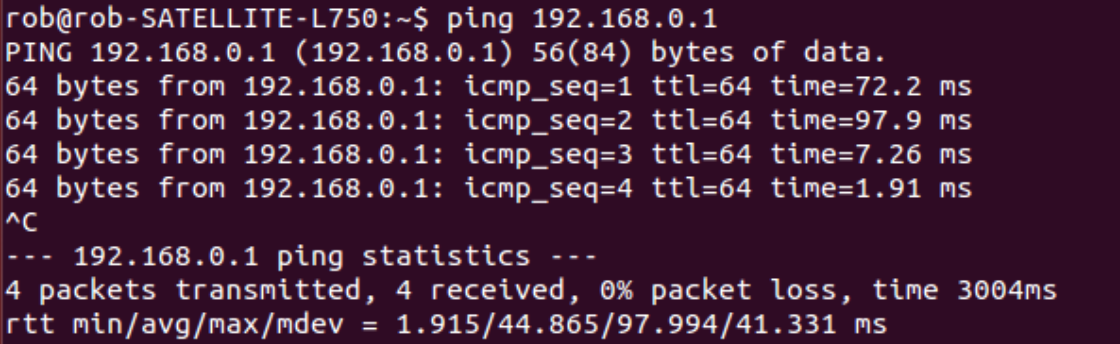
\includegraphics[width=7cm]{Figures/ping.png} }}%
    \qquad
    \subfloat[Receiving data using \lstinline{log_to_file}]{{\includegraphics[width=7cm]{Figures/Receiving.png} }}%
    \caption{Using \lstinline{ping} \& \lstinline{log_to_file} to send and receive ICMP packets between Archer C6 router and laptop}%
    \label{fig:UbuntuTerminals}%
\end{figure}
Hence, I was able to present one packet's SNR and CSI-phase across the 30 subcarriers once the data was converted to absolute units. Each stream conveys similar information as seen by each coloured trace. However, there isn't enough information to understand anything about the surrounding environment. 
\begin{figure}[H]%
    \centering
    \subfloat[CSI amplitude of each stream for one packet]{{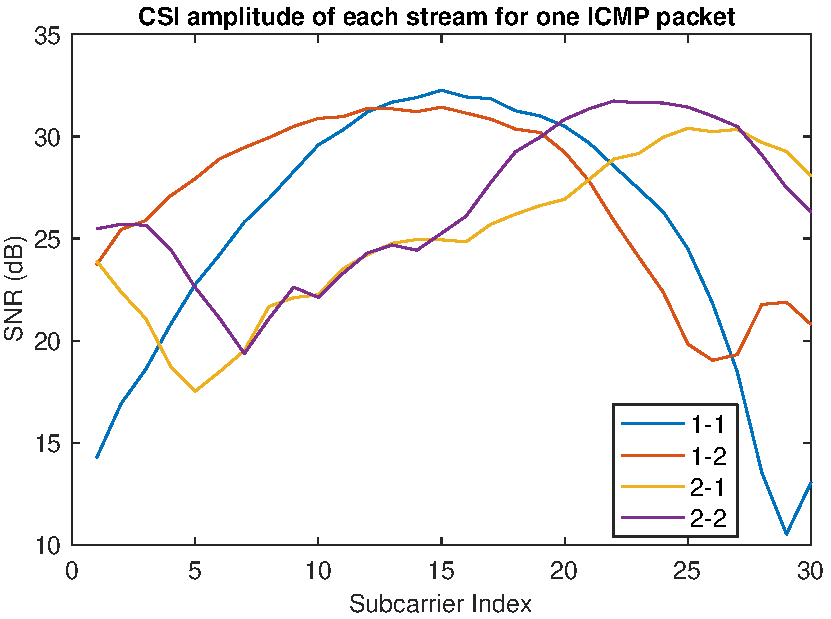
\includegraphics[scale = 0.5]{Figures/CSI_amplitude_subcarriers.pdf} }}%
    \qquad
    \subfloat[Wrapped phase of each stream for one packet]{{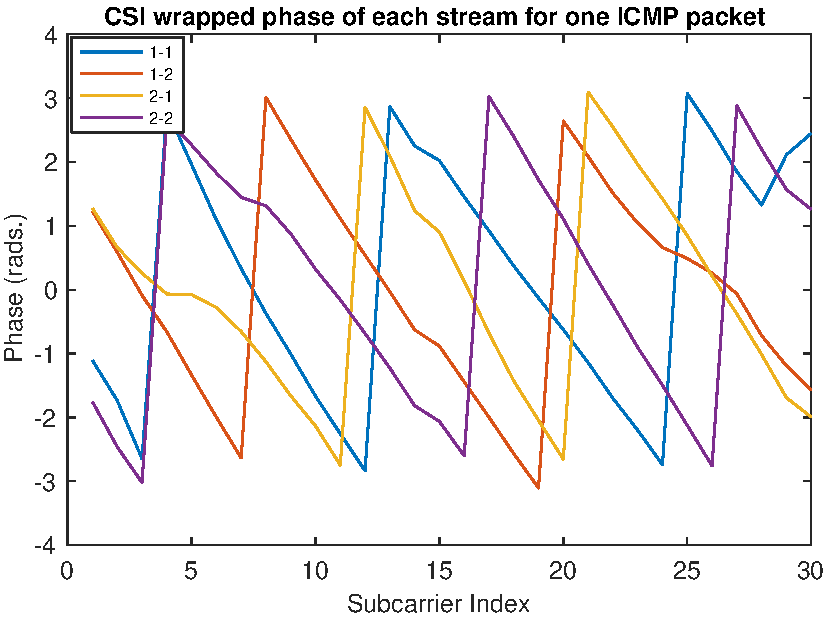
\includegraphics[width=7cm]{Figures/CSI_phase_subcarriers.pdf} }}%
    \caption{($2\times 2$ MIMO-OFDM system) CSI amplitude experiences frequency dependent fading at the edges of the channel bandwidth (Subcarriers 1 and 30). CSI phase is wrapped between $\pi$ and $-\pi$ rads. in a typical '$zig-zag$' pattern}%
    \label{fig:CSIAMPLITUDE&PHASE}%
\end{figure}
The CSI phase can be unwrapped using \lstinline{unwrap} in MATLAB to verify the phase according to RT-Fall and \cite{perceivingAccurateCSI}. It was decreasing for each consecutive subcarrier.
\begin{comment}\begin{figure}[H]
    \centering
  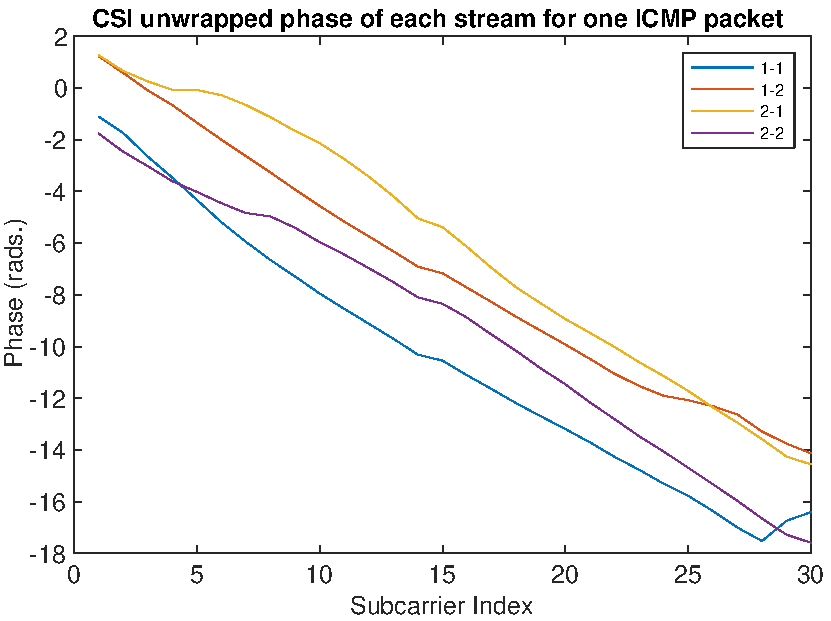
\includegraphics[scale=0.5]{Figures/CSI_unwrapped_subcarriers.pdf}
  \caption{CSI unwrapped phase for each of the 4 streams is presented correctly as descending for all 30 subcarriers}
  \label{fig:unwrappedPhase}
\end{figure}\end{comment}
However, each stream has 30 values per packet. A link between each of these needed to be found to simplify the calculations:
\begin{figure}[H]%
    \centering
    \subfloat[Different Streams for Subcarrier 15]{{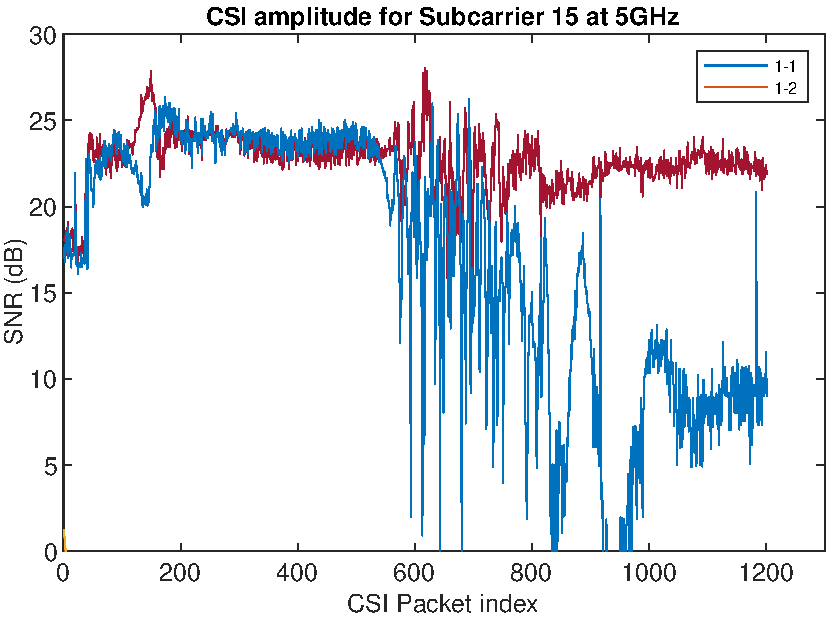
\includegraphics[scale = 0.5]{Figures/subcarrier15.pdf} }}%
    \qquad
    \subfloat[Different subcarriers in Stream 1-1]{{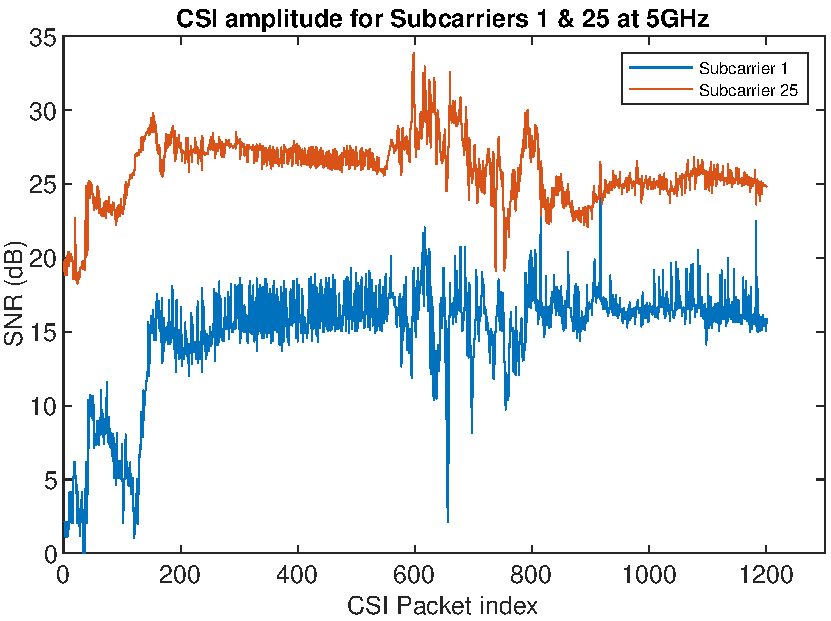
\includegraphics[scale=0.5]{Figures/differentSubcarriers.pdf} }}%
    \caption{Demonstrating that different streams react differently to human activity in (a) but different subcarriers in the same stream act similarly in (b)}%
    \label{fig:subcarriersVSstreams}%
\end{figure}
In Figure 4.4 (a), the fall occurring at the 600th packet affects streams 1-1, 1-2 differently due to the large change in the blue plot compared to red. However, human activities affect subcarriers similarly as seen in Figure 4.4 (b). This allows me to use the Equation \ref{eqn:3.1} to average the subcarriers into 1 value for each stream. 
\section{Data Processing}
\subsection{CSI Amplitude}
%%%%%%%%%%%%%%%%%%%%%%%%%%%%%%
The result of using Eqn. \ref{eqn:3.1} is shown below where the 30 subcarriers shown in Fig. 4.4 (a) are calculated and converted to one value per packet in Fig. 4.4 (b). The overall shape of the subcarriers is preserved but the full SNR range is not (some subcarriers have values around 27dB while Fig 4.5 (b)'s maximum point is 25dB). This implies a loss of frequency diversity in the calculation making it problematic for fall detection as seen by WiFall.
\begin{figure}[H]%
    \centering
    \subfloat[Subcarrier amplitudes in Stream 1-1]{{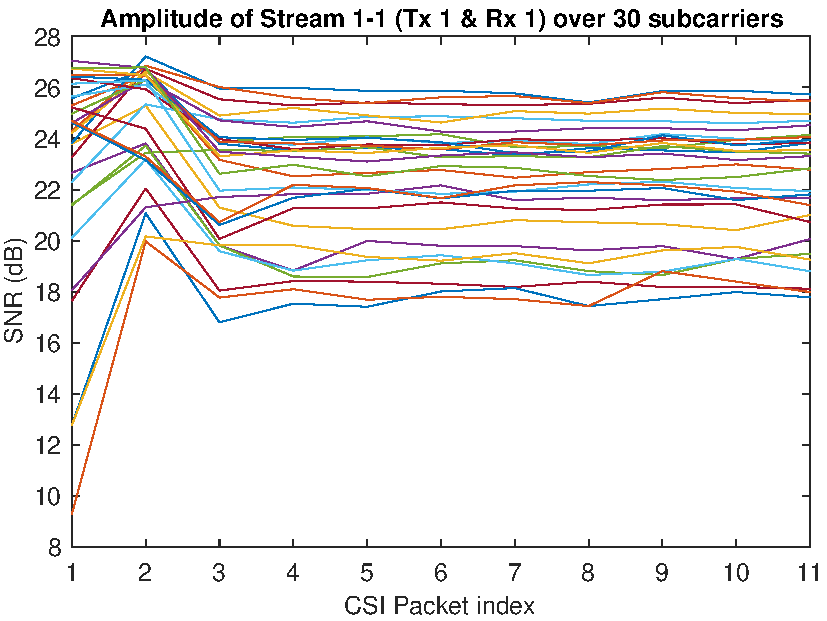
\includegraphics[scale = 0.5]{Figures/onlytaking10.pdf} }}%
    \qquad
    \subfloat[Averaged amplitude. One value per packet]{{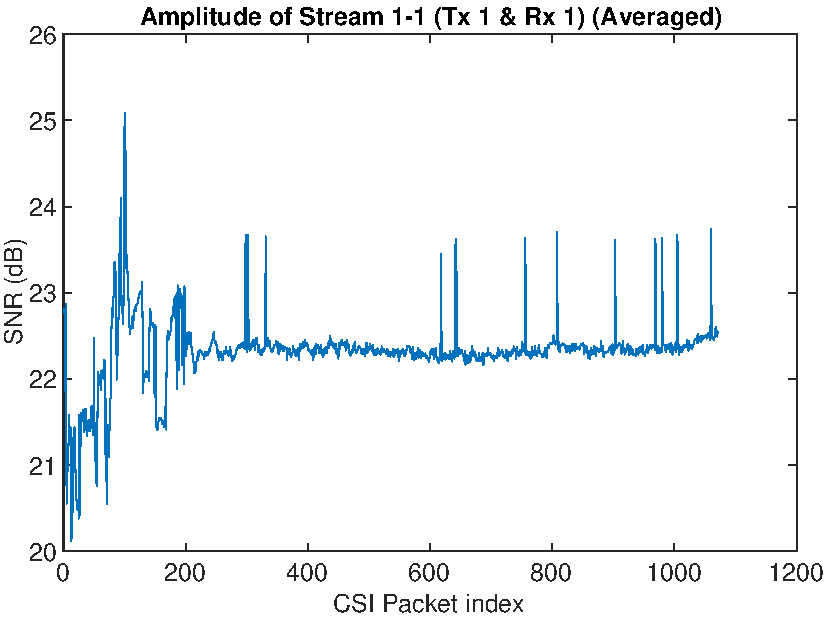
\includegraphics[scale=0.5]{Figures/averagedForAmplitude.pdf} }}%
    \caption{Using the findings from Fig. \ref{fig:subcarriersVSstreams}, I apply Eqn. \ref{eqn:3.1} to obtain a simpler plot in (b)}%
    \label{fig:applyingAmplitudeEquation}%
\end{figure}
\vspace{11pt}
\begin{figure}[H]
\centering
\begin{tabular}{cc}
  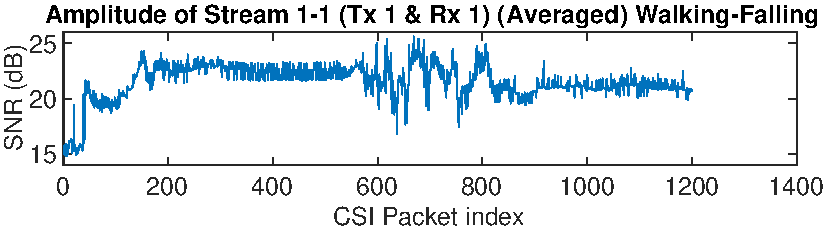
\includegraphics[scale = 0.5]{Figures/walkingFallingAveraged.pdf} &   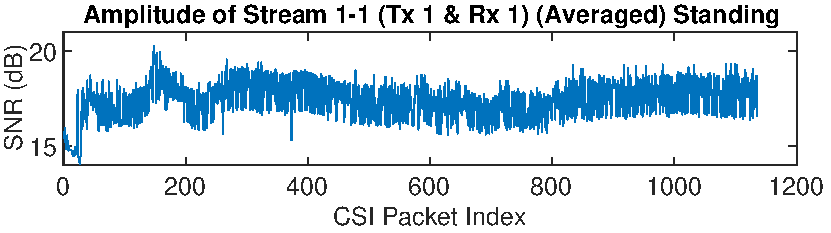
\includegraphics[scale=0.5]{Figures/standingForAmplitude.pdf} \\
(a) Person falling (600th packet) & (b) Person standing still \\[6pt]
\multicolumn{2}{c}{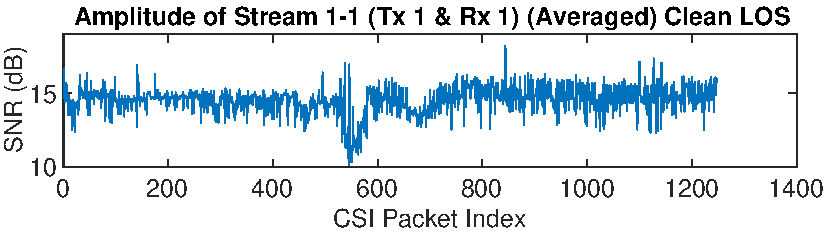
\includegraphics[scale = 0.5]{Figures/cleanLOSForAmplitude.pdf} }\\
\multicolumn{2}{c}{(c) Clean LOS from Tx-Rx}
\end{tabular}
\caption{CSI amplitude with with person falling, standing and then being absent (Clean LOS)}
\label{fig:diffamplitudes}%
\end{figure}
I carried out a number of tests using the averaged CSI amplitude as shown in Fig. 4.5. Mobile and immobile activities obtain different CSI amplitude variance with time. It is clear in (a) that something has occurred but this "fall" could also be confused with the fluctuation in (c) caused by the small disturbance closer to the receiver with nobody in the environment. It is hard to differentiate and recognise patterns between each of the situations. 
\subsection{CSI Phase}
I have noticed that CSI phase is more granular indication of a fall in an environment. I plotted the phase difference, as noted in PhaseU \citep{PhaseU}, below:
\begin{figure}[H]
    \centering
    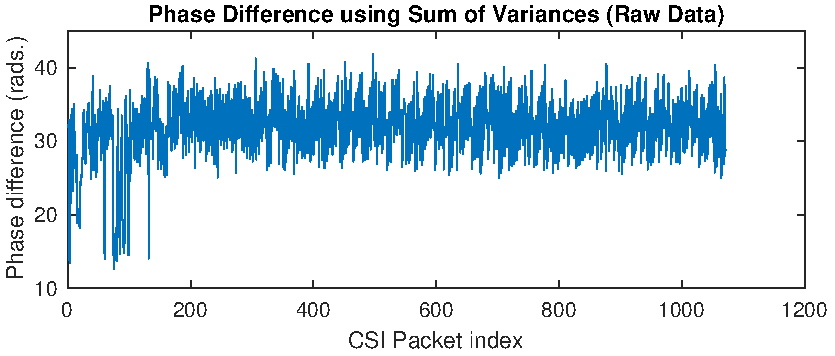
\includegraphics[scale=0.75]{Figures/uncleanPhaseFallCLASSROOM.pdf}
    \caption{Phase difference containing phase offsets and outliers}
    \label{fig:uncleanPhaseDiff}
\end{figure}
This plot above contains the unknown phase offset and timing offset as alluded to in Eqn. \ref{eqn:3.3} \& \ref{eqn:3.4}. No recognisable patterns in the data are noticeable. Using Eqn. \ref{eqn:3.5}, I can obtain a cleaner plot:
\begin{figure}[H]
    \centering
    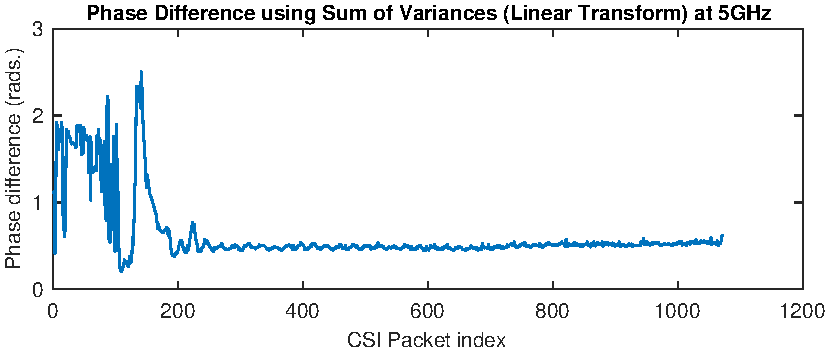
\includegraphics[scale=0.75]{Figures/cleanPhaseFallCLASSROOM.pdf}
    \caption{Phase difference from Fig. 4.7 after applying linear transform in Eqn. \ref{eqn:3.5}.}
    \label{fig:cleanerPhaseDiff}
\end{figure}
This plot has all phase offsets and outliers removed. The data is now interpretable in the time domain and human activities can be noticed. 
\subsection{Phase Difference \& Amplitude for Fall Detection}
Clearly, I have demonstrated the phase difference is a much more granular indicator of a human activity in an environment. I tested this using a "walking-fall" as shown below:
\begin{figure}[H]
    \centering
    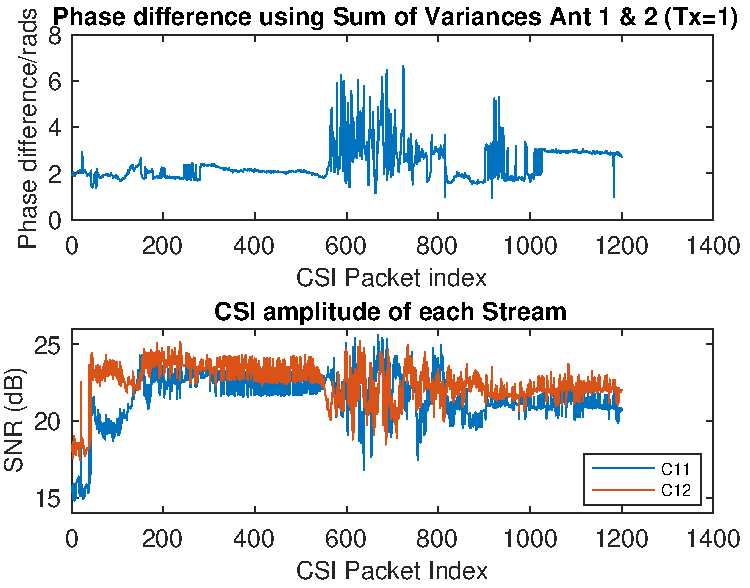
\includegraphics[scale=0.75]{Figures/subplotFall.pdf}
    \caption{CSI amplitude and transformed phase difference for 4m environment between Tx and Rx with a person walking into the environment, falling and standing up again. }
    \label{fig:finalPlot}
\end{figure}
Both the amplitude and phase difference experience a sudden disturbance on start up. This is a combination of the rate selection algorithm of the Archer C6 router adjusting and the test subject walking close to the receiver creating a multipath environment. The fall occurring just before the 600th packet creates a very large disturbance in the phase difference. The CSI amplitude suffers a disturbance also. However, the amplitude's response to the fall is very similar to the disturbance caused by the person walking between the 200th and 400th packet. The amplitude can be used for activity detection as in WiFall but isn't clear enough for fall detection. The phase difference clearly shows where the fall finished, save for a few oscillations. It is a much more sensitive indicator and the transformed phase is much less noisy than the amplitude. In a more complex MIMO-OFDM system, the phase difference resolution will improve due to the introduction of more antennas into the system and thus, performance for LOS/NLOS environments will greatly improve.

\chapter{Future Work}\label{chapter:Future Work}
\section{Signal Processing}
Up until now, I have researched and implemented many different pre-processing techniques which has led to the CSI amplitude and phase data being more interpretable. The lack of synchronisation between transmitter and receiver as mentioned in Section 2.2.3 presents two issues: The sampled CSI data may not be continuous which is needed for feature extraction during a fall and I am unable to obtain a spectrogram of the data if they are unevenly spaced in the time domain. Feature extraction is extremely hard and inaccurate with this issue. To resolve this, I will implement a \textbf{1-D linear interpolation algorithm} on the raw CSI. This is done in MATLAB using \lstinline{interp1} on each transmitter-receiver pair matrix ($CSI_{ij}$). This will allow me to see accurate receiving times for each packet.\par
To make the training of my classifiers easier, I can perform band-pass filtering on the interpolated CSI data. This can filter out the lower frequency components as seen by RT-Fall in the range [0,4]$Hz$ as most fall or fall-like activities occur in the range [5,10]$Hz$ \citep{RTFall}.
\section{Activity Segmentation}
Having obtained real-life CSI data from an indoor environment of over 10mins to mimic a real test environment such as a bedroom, I need to find the finishing point of a fall or fall-like activity in this large amount of CSI data. I will use a \textbf{threshold-based sliding window} firstly. I will need two stable signal streams across multiple sliding windows from which I can calculate their mean $\mu$ and normal standard deviation $\sigma$. I can calculate if an equation involving these is less than a threshold value detecting their current state (stable/fluctuating).\par
When there is a transition in signal state, I can mark this time as the \textit{start} and the time of another transition as the \textit{end} which gives me an activity window. From here, I can segment the activities by determining the appropriate trace back window size. 
\section{Feature Extraction \& Classification}
As seen in RT-Fall and WiFall, which use similar number and type of features for recognising a fall, I will need to gather and research further features that could be an indication of a fall occurring in the CSI data. All of these features will form the input to my classifiers for training the classification model. \par
I will then be able to design a binary classifier such as a SVM (Support Vector Machine) for detecting between a fall and a fall-like activity as these are the most similar activities and could lead to the highest missed/false detection rate. The training dataset will need to be created in a usual living room and the human activities will need to be segmented, labelled and passed into the SVM classifier along with the extracted features. With user feedback, classification errors will be relabelled to adjust the model. I can then test the model again with unseen data. \par 
I am hoping to implement a similar method using a Decision Tree Classifier such as RandomForest and perhaps, a Neural Network, if time allows and the classification accuracy from SVM is not high enough. 
\begin{comment}If I have enough time, I would like to investigate if the CSI.dat files are populated in real time and if there is a possibility of creating a Real Time system out of my work. \par \end{comment}
Currently, I am in the process of extensive \& prolonged CSI data gathering for the activity segmentation step and the enhanced data pre-processing involving interpolation and filtering. 

%\chapter{Conclusion}\label{chapter:Conclusion}
%\input{Chapters/Chapter6_Conclusion.tex}

\begingroup
    \singlespacing
    \bibliographystyle{abbrvnat}
    \bibliography{References}
    \setcitestyle{authoryear,open={(},close={)}}
\endgroup

\newpage

\appendix
%In this section I can add any code which was used to generate any of the cleaner plots/obtain the plots from the CSI Data
%Put in any of the code that was used for the amplitude and the phase of each for just a 1x2 SIMO now
%Look at listings.sty to see how to include the matlab code
%\addcontentsline{toc}{chapter}{Appendix}
%\chapter{My First Appendix}\label{chapter:Appendix A}
%In this file (Appendices/Appendix$\_$A.tex) you can add appendix chapters, just as you did in the Document.tex file for the `normal' chapters.
You can also choose to include everything in this single file, whatever you prefer.

\end{document}